\section{Auswertung}
\label{sec:Auswertung}
%Fehlerrechnung
Für die Auswertung der Messergebnisse wird im Folgenden der Mittelwert immer als
\begin{equation}
  \bar{x} = \frac{1}{N}\sum_{i=1}^{N} x_{i}
\end{equation}
berechnet und die Standardabweichung mit
\begin{equation}
  \Delta\bar{x} = \frac{\sigma}{\sqrt{N}} = \sqrt{\frac{1}{N(N-1)}\sum_{i=1}^{N} (x_{i} - \bar{x})^2}.
\end{equation}
Weiterhin wird die Gaußsche Fehlerfortpflanzung
\begin{equation}
  \Delta f = \sqrt{\left(\frac{\partial f}{\partial x}\Delta x\right)^2 + \left(\frac{\partial f}{\partial y}\Delta y\right)^2 + \dots}
\end{equation}
verwendet. Für Plots und Regression wird Python genutzt.
%------------

%Figur einbinden
\begin{figure}
  \centering
  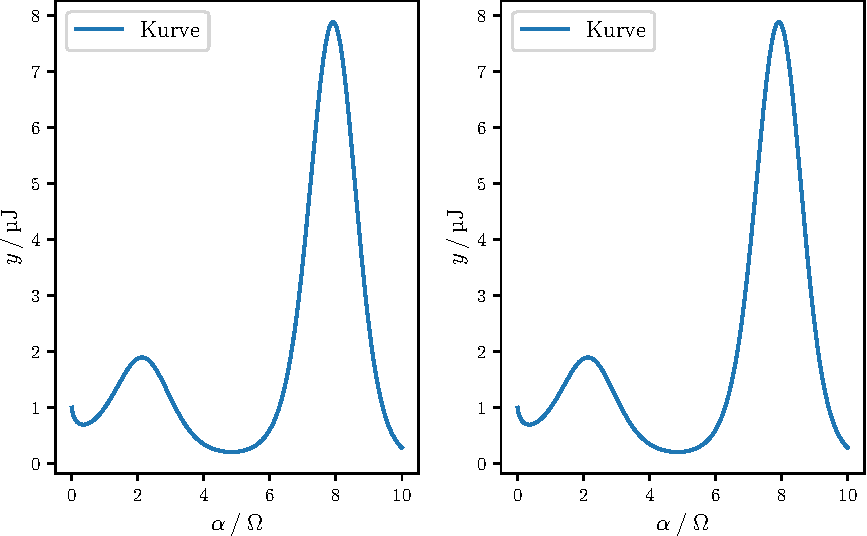
\includegraphics{plots/plot.pdf}
  \caption{Plot.}
  \label{fig:plot}
\end{figure}
%------

%Tabelle einbinden
\begin{table}
  \centering
  \caption{Beschreibung}
  \label{tab:Beispiel}
  \begin{tabular}{S[table-format=2.0] S[table-format=2.2]}
    \toprule
    {$f \:/\: \si{\kilo\hertz}$} & {$U_C \:/\: \si{\volt}$}\\
    \midrule
50  & 4.08\\
52  & 3.76\\
  \end{tabular}
\end{table}
